\section{Architekturentscheidung}\label{arch_decission} \thispagestyle{nomarkstyle}
Nach einer sorgfältigen Analyse der unterschiedlichen Technologien wurde eine Architektur entworfen, welche in \cref{fig:webshop_arch} dargestellt ist. Die Komponenten wurden so gewählt, dass sie untereinander mit möglichst wenig Konfigurationsaufwand reibungslos funktionieren.

\begin{figure}[th!]
	\centering
	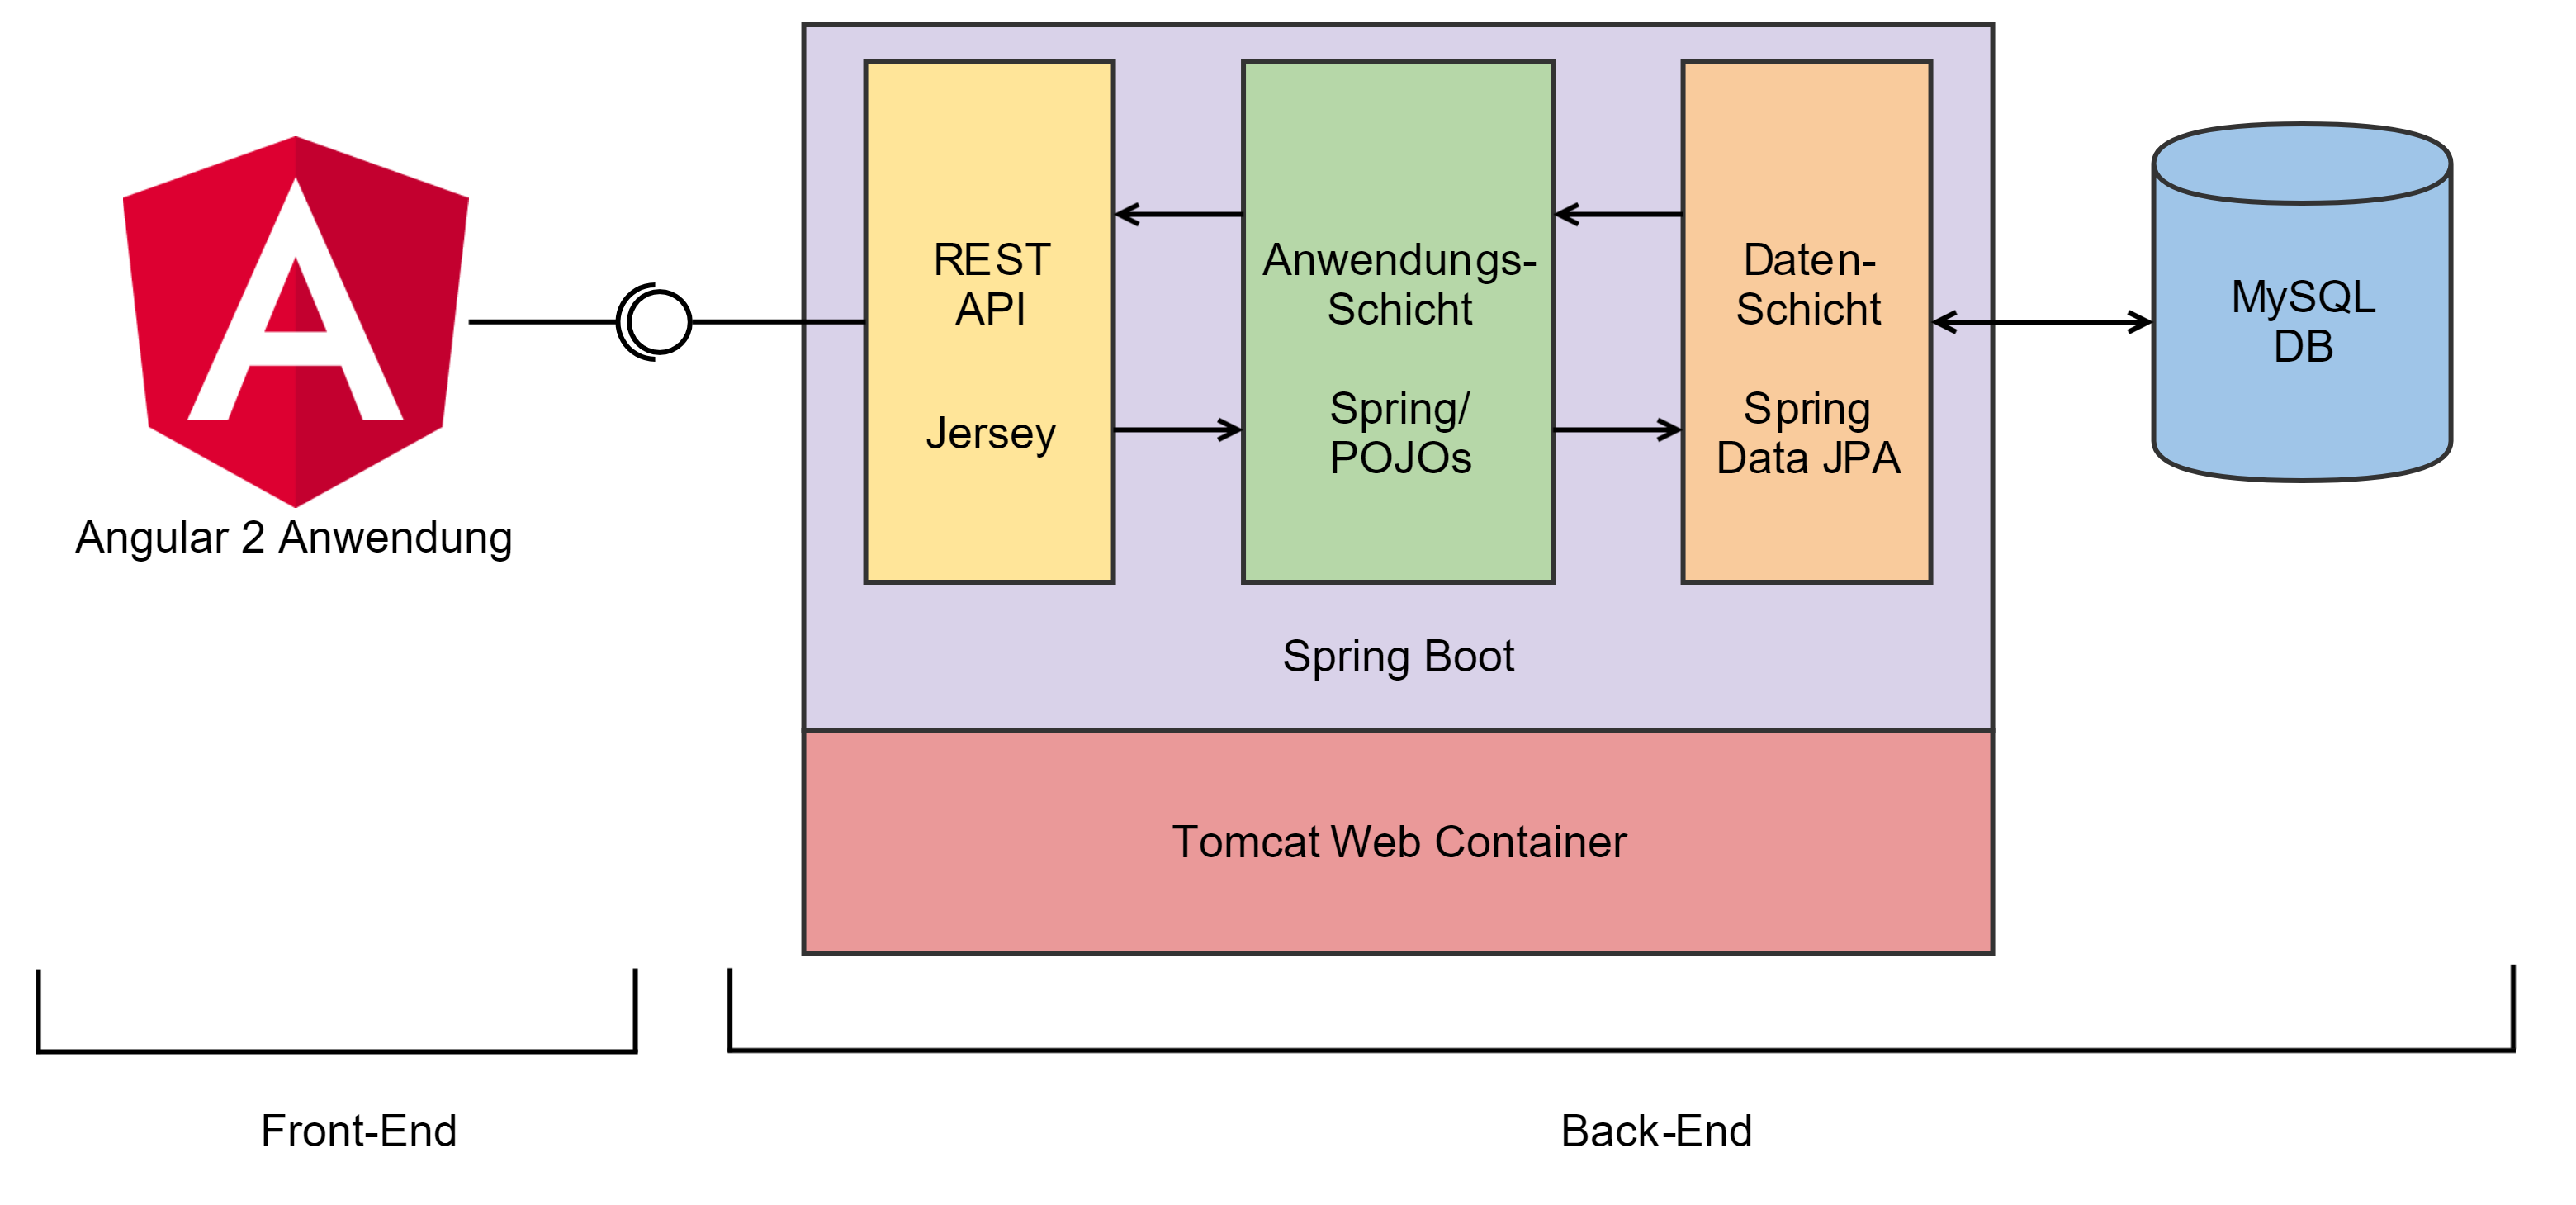
\includegraphics[width=\linewidth]{bilder/kap5/webshop_arch.png}
	\caption{Grundlegende Architektur des Webshops}
	\label{fig:webshop_arch}
\end{figure}

Im Folgenden werden die theoretischen Grundlagen zu den einzelnen Komponenten, sowie weitere Erläuterungen zu den Gründen der Architekturentscheidung beschrieben.

\subsection{Spring Boot Anwendung}
Spring ist ein Framework für die Entwicklung von Applikationen in der Programmiersprache Java.
Das Framework kann für alle Arten von Java-Anwendungen genutzt werden, da eine große Vielfalt an Abhängigkeiten für die unterschiedlichsten Funktionalitäten zur Verfügung steht.

Ursprünglich entstand Spring als eine leichtgewichtige Alternative zur Java Enterprise Edition (\acs{JEE}), sodass die Komponenten der Software nicht mehr als Enterprise JavaBeans (\acs{EJB}s) sondern als einfache Java Objekte (\acs{POJO}s) realisiert werden können.
Die Eigenschaften von \acs{EJB}s werden anhand von Techniken wie Dependency Injection und aspektorientierter Programmierung erreicht.
Ein großer Nachteil hierbei ist jedoch der große Konfigurationsaufwand für den Entwickler.
Initial erfolgte diese Konfiguration über mehrere \acs{XML}-Dateien. Ab Spring 2.5 wurde die \acs{XML}-basierte Konfiguration teilweise durch sogenannte Annotationen in den Java-Klassen ersetzt, was den Aufwand jedoch nicht sonderlich reduziert \cite{Walls2015}.

Das Ziel des Spring Boot Projekts ist es genau diesen Nachteil zu beseitigen. Durch eine automatische Konfiguration können Entwickler schnell komplexere Spring-Anwendungen aufbauen, ohne auf die Konfiguration von allgemeinen Funktionalitäten achten zu müssen.
Zudem ist auch das Einbinden von Spring-Abhängigkeiten stark vereinfacht \cite{Webb2013}.

Für die Verwendung von Spring Boot als serverseitiger Anwendung des Webshops spricht vieles.
Zum einen ist im Team bereits einige Erfahrung aus anderen Projekten vorhanden, die hier wiederverwendet werden kann.
Zum anderen erleichtert Spring Boot durch das einfache Aufsetzen der Anwendung, der umfangreichen Dokumentation, sowie der großen Auswahl an Abhängigkeiten deutlich den Start mit der Umsetzung der eigentlichen Anforderungen.
Besonders die Abhängigkeit \texttt{spring-boot-starter-web} ist für die Entwicklung von Webanwendungen nützlich, denn damit wird automatisch ein Webserver bzw. ein Java Servlet Container (Apache Tomcat) in das Projekt eingebettet.

\subsection{Angular 2 Frontend}\label{angular_arch}

Angular 2 ist die neue, komplett umgebaute Version des Angular 1.x Frameworks (auch bekannt als AngularJS).
Diese Version liefert eine brandneue Architektur basierend auf Komponenten die in TypeScript implementiert werden.
Bei TypeScript handelt es sich wiederum um ein von Microsoft entwickeltes Superset von JavaScript.
TypeScript führt ein optionales Typsystem ein, sowie mehrere ECMAScript 6 Funktionalitäten, wie zum Beispiel Unterstützung von Interfaces, Klassen und Vererbung.
Der Vorteil dabei ist, dass die Erweiterungen von TypeScript von einem Compiler in herkömmliches JavaScript umgewandelt werden, sodass man TypeScript mit jedem Browser oder auch mit Node.js benutzen kann, solange der Code vorher kompiliert wird \cite{Deeleman2016}.

Bei Angular 2 handelt es sich um ein sehr junges Framework (die endgültige Version wurde im September 2016 veröffentlicht), sodass es noch zu früh ist um dessen Erfolg messen zu können.
Fest steht jedoch, dass die aktuelle Beliebtheit von TypeScript ein ausschlaggebender Faktor für den Erfolg sein könnte.
Da im Rahmen dieses Projekts allgemein keine bestimmten Technologien vorgegeben wurden, bietet es sich durchaus an, das Framework mit den neuen Features und der neuen Architektur näher kennenzulernen.

Neben dem eigenen Interesse an diesem Framework sprach noch ein weiterer Faktor maßgeblich für die Entscheidung, Angular als Technologie für die Implementierung des Frontends zu verwenden.
Es ist geplant, den Webshop als eine Single Page Application zu realisieren, deren Vorteile bereits in \cref{web_types} geschildert wurden.
Angular gehört schon seit der ersten Version zu den beliebtesten Frameworks für diesen Anwendungsfall, da die mitgelieferten Tools und Funktionalitäten die Implementierung sehr vereinfachen.
Besonders der Routing-Mechanismus für die Navigation in der \acs{SPA} ist in Angular sehr ausgereift.

In den nächsten Seiten werden die Eigenschaften des Frameworks etwas ausführlicher behandelt, da das Thema im Laufe der Implementierung mitunter den größten Einarbeitungsaufwand betrug.

Eine Angular 2 Anwendung besteht im Grunde aus den folgenden Bausteinen\cite{Angular.io2017}:

\begin{itemize}
	\item \textit{Komponenten}
	\item \textit{Templates} 
	\item \textit{Metadaten}
	\item \textit{Modulen}
	\item \textit{Data Binding} 
	\item \textit{Direktiven}
	\item \textit{Services}
	\item \textit{Dependency Injection}
\end{itemize}

\subsubsection{Komponenten}
Komponenten sind TypeScript-Klassen, die die Darstellung der Oberfläche, die sogenannte \enquote{View} kontrollieren.
Jede Klasse enthält Attribute und Methoden, mit denen die Darstellung verändert werden kann.

\subsubsection{Templates}
Templates definieren wie die Darstellung einer Komponente genau aussieht.
Hierfür wird eine erweiterte Form von \acs{HTML} verwendet. Templates können somit zum Beispiel auch Kinder einer Komponente durch besondere HTML-Tags einbinden.

\subsubsection{Metadaten}
Metadaten geben Angular Information darüber, wie eine Klasse verarbeitet werden soll. Komponenten können erst von Angular als solche erkannt werden, wenn die Klasse die entsprechenden Metadaten enthält.
In TypeScript wird das mittels einem Decorator gemacht, eine Annotation, die über die Klassendeklaration gesetzt wird.
\\
\begin{lstlisting}[language=JavaScript,caption={Beispiel Metadaten-Annotation für Komponenten},label=lst:metadata_ex]
@Component({
selector:    'sample-component',
templateUrl: './sample.component.html',
providers: []
})
export class SampleComponent implements OnInit {
/* . . . */
}
\end{lstlisting}

In \cref{lst:metadata_ex} ist als Beispiel die Annotation für Komponenten dargestellt. Unter \texttt{@Component} können unterschiedliche Aspekte einer Komponente definiert werden, wie der \acs{HTML}-Selektor, der Ablageort des Templates oder benötigte Abhängigkeiten.

\subsubsection{Module}
Module fassen mehrere Komponenten und Services zu einem Funktionalitäts-Block zusammen. Jede Angular Anwendung besitzt mindestens ein Modul, das sogenannte \enquote{Root Module}.
\\
\lstinputlisting[language=JavaScript,caption=Root Modul,label=lst:root-module]{listings/app.module.ts}

\cref{lst:root-module} zeigt den initialen Zustand eines Root-Moduls. Jedes Modul wird durch die Metadaten in der \texttt{@NgModule}-Annotation definiert.
Diese teilt Angular mit, welche Komponenten im Modul deklariert sind, sowie welche Module und Services die importiert bzw. eingebunden werden müssen.
Das Root-Modul enthält zusätzlich auch die \texttt{bootstrap}-Definition, in der die Hauptkomponente festgelegt wird, die Angular beim Ausführen der Anwendung in die \texttt{index.html} der Webseite einfügt \cite{Angular.io2017a}.

\subsubsection{Data Binding}
\begin{wrapfigure}[9]{r}{0.4\textwidth}
	\centering
	\vspace{-20pt}
	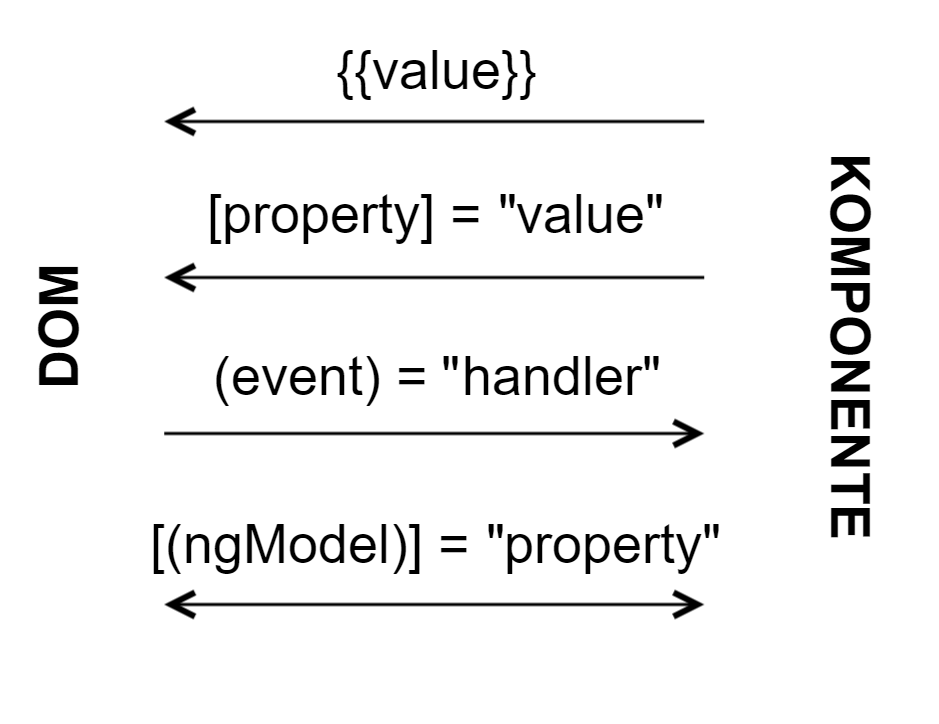
\includegraphics[width=0.4\textwidth]{bilder/kap5/databinding}
	\vspace{-20pt}
	\caption{Arten des Data Bindings in Angular 2}
	\label{fig:databinding}
\end{wrapfigure}
Als Data Binding (zu Deutsch Datenbindung) bezeichnet man den Mechanismus zur Zuordnung von bestimmten Elementen eines Templates zu Datenstrukturen der dazugehörigen Komponente.
\cref{fig:databinding} zeigt die vier Arten von Data Binding Syntax in Angular.
Jede Form von Data Binding hat auch eine Richtung: von der Komponente zum Document Object Model (\acs{DOM}) im Template, vom \acs{DOM} zur Komponente oder bidirektional.

\newpage
Um diese vier Data Binding Formen weiter zu veranschaulichen, ist in \cref{lst:databinding_ex} jeweils ein Beispiel dargestellt. In der ersten Zeile wird durch die doppelte geschweifte Klammern der Wert \texttt{name} vom Attribut \texttt{user} der Komponenten-Klasse in die \acs{DOM} eingefügt.
Zeile 2 zeigt eine eingebundene Kindkomponente \texttt{FoodComponent}, die als Input den Wert des Attributs \texttt{selectedFood} von der Komponenten-Klasse erhält.
Die runden Klammern mit einem Event-Bezeichner in Zeile 3 binden eine Methode der Komponente zum angegebenen Event.
Die letzte Zeile zeigt eine besondere Art von Data Binding, das \textit{Two-Way Data Binding}.
Hierbei fließt der Wert vom Attribut der Klasse nicht nur von der Komponente in die \acs{DOM} ein, sondern wird auch in der Komponente aktualisiert wenn dieser sich beispielsweise durch eine Benutzereingabe verändert.
\\
\begin{lstlisting}[language=HTML5,caption={Beispiele zu den Data Binding Arten},label=lst:databinding_ex]
<h1>Hallo {{user.name}}</h1>
<food-component [user]="selectedFood"></food-component>
<li (click)="selectFood(food)"></li>
<input [(ngModel)]="user.name">
\end{lstlisting}

\subsubsection{Direktiven}
Bei Direktiven handelt es sich um Klassen mit dem \texttt{@Directive}-Decorator, in denen beliebige Funktionalitäten zur dynamischen Transformation der DOM definiert werden können.
Komponenten sind sozusagen Direktiven mit einem Template. Neben Komponenten gibt es aber auch zwei andere Arten von Direktiven: strukturelle und Attribut-Direktiven.
Erstere verändern das Layout der View durch das Hinzufügen, Löschen oder Ersetzen von Elementen in der \acs{DOM}.
Attribut-Direktiven verändern hingegen das Aussehen oder das Verhalten eines bereits vorhandenen DOM-Elements.
Ein Beispiel dafür ist die \texttt{ngModel}-Direktive die bereits in \cref{lst:databinding_ex} gezeigt wurde.

\subsubsection{Services}
Der Begriff Service ist in Angular sehr weit umfassend, da grundsätzlich alles mögliche ein Service sein kann.
Typischerweise handelt es sich jedoch einfach um eine Klasse, die eine konkrete Aufgabe erledigt, wie zum Beispiel Logging, Datenzugriff, Berechnungen, usw.
Diese Logik sollte idealerweise nie in Komponenten selbst enthalten sein, da diese nur als Mediatoren zwischen der Darstellung (View) und der Logik zu verstehen sind.

Services zeigen an sich also keine besondere Angular-Eigenschaften. Um die Trennung zwischen der in Services gekapselten Logik und den Komponenten einfach zu überwinden, wird jedoch ein charakteristischer Mechanismus von Angular verwendet, die Dependency Injection.

\subsubsection{Dependency Injection}
Dieser Mechanismus ermöglicht es, eine neue Instanz einer Klasse mit allen nötigen Abhängigkeiten (in der Regel Services) zu versorgen.
Um Angular mitzuteilen, welche Services eine Komponente benötigt, müssen diese im Konstruktor oder alternativ im \texttt{@Component}-Decorator deklariert werden, wie in \cref{lst:metadata_ex} bereits gezeigt wurde.

\subsection{REST Services}
Für die Kommunikation zwischen Front- und Backend wird REST eingesetzt. REST steht für Representational State Transfer und ist ein Architekturstil für den Entwurf von verteilten Systemen. Die Grundlage von REST wird durch folgende sechs Prinzipien festgelegt \cite{Varanasi2015}:

\begin{itemize}
	\item \textit{Client-Server}. Die Unterteilung zwischen Client und Server ermöglicht es den jeweiligen Komponenten sich unabhängig voneinander zu entwickeln und erlaubt dementsprechend die Skalierung des Systems.
	\item \textit{Zustandslos}. Die Kommunikation zwischen Client und Server sollte zustandslos sein. Das bedeutet, dass der Server sich nicht den Zustand des Clients merken braucht. Stattdessen kümmert sich der Client darum, alle notwendigen Informationen in der Anfrage mitzuliefern, damit der Server diese verstehen und verarbeiten kann.
	\item \textit{Mehrschichtige Systeme}. Es können mehrere Schichten wie zum Beispiel Gateways, Firewalls oder Proxies zwischen Client und Server existieren. Diese Schichten können transparent hinzugefügt, modifiziert, umgeordnet oder gelöscht werden.
	\item \textit{Cache}. Antworten vom Server müssen als \enquote{cacheable} oder \enquote{noncacheable} deklariert sein. Dadurch wissen Clients, ob sie die Antworten zwischenspeichern können, um sie später wiederverwenden zu können. Dieser Vorgang verringert die Last auf dem Server und verbessert die Performance.
	\item \textit{Uniform Interface}. Alle Interaktionen zwischen Client, Server und dazwischenliegenden Komponenten basieren auf der Uniformität der Schnittstellen. Solche Schnittstellen definieren welche Ressourcen über eine eindeutige \acs{URI} durch bestimmte \acs{HTTP}-Methoden erreichbar sind. Ein Beispiel für eine REST URI könnte folgendermaßen aussehen: \\
	\texttt{http://blog.example.com/posts/1}\\
	Die URI repräsentiert hier den Zugriff auf einem Blog-Post mit Identifikator 1.
	\item \textit{Code on demand}. Clients können ihre Funktionalitäten erweitern, indem sie Code (wie JavaScript Skripte oder Java Applets) bei Bedarf herunterladen und ausführen. Dies ist jedoch eine optionale Eigenschaft.
\end{itemize}

Anwendungen die diese Prinzipien befolgen, gelten als \enquote{RESTful}, also REST-konform. Es ist hierbei nicht vorgegeben, welche Technologie konkret für die Entwicklung solcher Anwendungen benutzt werden soll.
Theoretisch ist es möglich eine REST-Anwendung mit einer beliebigen Netzwerk-Infrastruktur oder einem beliebigen Protokoll aufzubauen.
In der Praxis nutzen diese Applikationen jedoch hauptsächlich die Eigenschaften der Web-Entwicklung und verwenden dementsprechend \acs{HTTP} als Übertragungsprotokoll.

Von den sechs oben beschriebenen Punkten ist das Prinzip des Uniform Interfaces das Hauptmerkmal von REST-Anwendungen, welches diese Art von Applikationen von anderen netzwerkbasierten Anwendungen unterscheidet.

\subsection{MySQL Datenbank}
Den Ausschlag für die Wahl eine MySQL-Datenbank gaben mehrere Faktoren. Zum einen ist MySQL weit verbreitet und bietet als Open Source-Projekt kostenfrei eine Vielzahl an Funktionalitäten.
Ein weiterer Punkt ist die bereits vorhandene Erfahrung im Umgang mit SQL aus vorigen Projekten.
Unter dem Gesichtspunkt der bisherigen Entscheidung für Java als Implementierungssprache für das Backend ist MySQL eine gute Wahl, da es entsprechende Treiber für die Ansteuerung gibt und die Java Persistence API (\acs{JPA}) eine gute Integration der Datenbank in die Anwendung ermöglicht.

\subsection{Hibernate ORM}
Mit Java und einer MySQL-Datenbank als Voraussetzung bietet sich die Verwendung von Hibernate für die Objektrelationale Abbildung an.
Mit Hibernate stehen dem Entwickler viele Annotationen zur Verfügung, die eine einfache Kennzeichnung von Klassen und Attributen für ihre Rolle in der Datenbank ermöglichen.
Auch bei komplexeren Strukturen wie einer Vererbungshierarchie von Klassen gewährleistet Hibernate eine Abbildung auf die Datenbankstruktur und bietet verschiedene Möglichkeiten an, wie das geschehen kann.
Außerdem können die Tabellen der Datenbank auch von Hibernate erzeugt werden, wenn das Modell über die Java-Klassen zuvor definiert wird.
